
% This LaTeX was auto-generated from MATLAB code.
% To make changes, update the MATLAB code and republish this document.

\documentclass{article}
\usepackage{graphicx}
\usepackage{color}

\sloppy
\definecolor{lightgray}{gray}{0.5}
\setlength{\parindent}{0pt}

\begin{document}

    
    

\section*{Farid Tavakkolmoghaddam HW4}

\begin{verbatim}
%Steering control
clear; close all; clc
T=50;
x0 =[0;1;pi/4]; % Feel free to change the initial state and sampling horizon.



% design steering control to follow a straight lane while maintaining a given velocity
% the lateral position yr= 2;



%TODO: param is the additional parameter to pass to the ode function.
[T,X] = ode45(@(t,x) ode_dubins(t,x), (0:T), x0);
tt=0:1:50;
XX=10*tt; % desired trajectory x
YY=2*ones(1,51); % desired trajectory y
thetta=2*zeros(1,51); % desired trajectory y

% plot your state trajectories for both 1 and 2, using the following code or else.
figure
title(' X position vs. time')
plot(T,X(:,1),'k',tt,XX,'b*','LineWidth',2);
xlabel('t (s)');
ylabel('x (m)','FontSize',12,'FontWeight','bold','Color','k');
legend('Actual','desired')
grid

figure
title(' Y position vs. time')
plot(T,X(:,2),tt,YY,'r--','LineWidth',2);
xlabel('t (s)');
ylabel('y (m)','FontSize',12,'FontWeight','bold','Color','k');
legend('Actual','desired')
grid

figure
title(' Orientation vs. time')
plot(T,X(:,3),tt,thetta,'r--','LineWidth',2);
xlabel('t (s)');
ylabel('theta (rad)','FontSize',12,'FontWeight','bold','Color','k');
legend('Actual','desired')
grid

figure ('name','X v.s y')
title(' x vs. y')
plot(X(:,1), X(:,2),'LineWidth',2)
xlabel('X (m)','FontSize',12,'FontWeight','bold','Color','k');
ylabel('Y (m)','FontSize',12,'FontWeight','bold','Color','k');
grid
\end{verbatim}

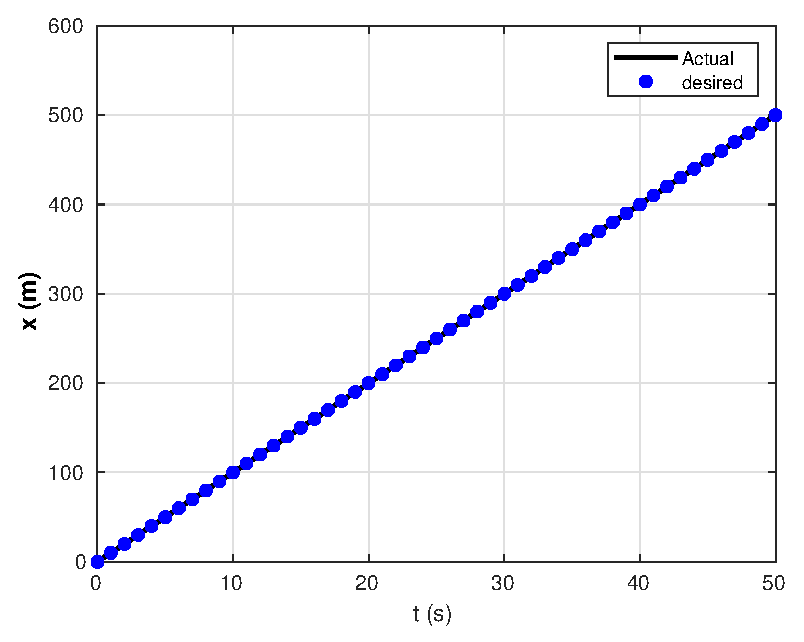
\includegraphics [width=4in]{vehicle_steering_01.eps}

\includegraphics [width=4in]{vehicle_steering_02.eps}

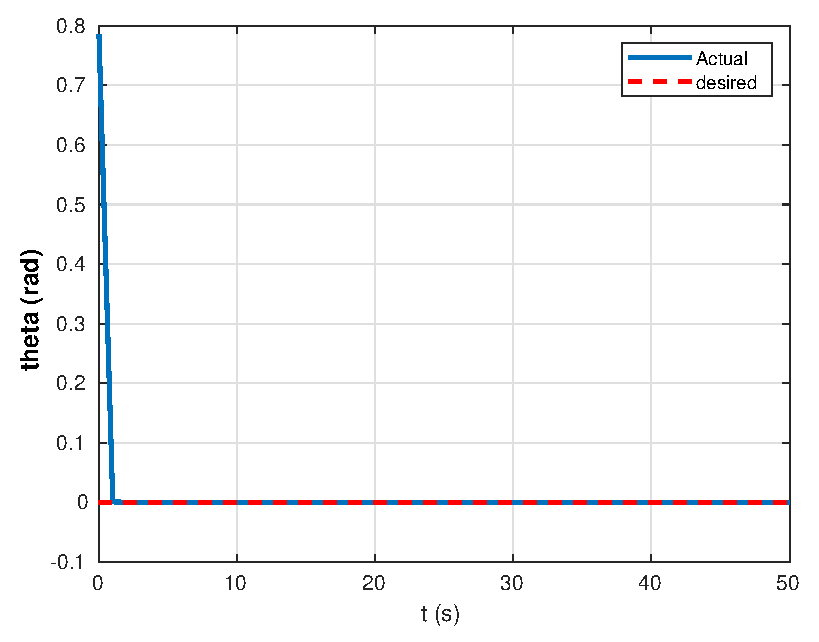
\includegraphics [width=4in]{vehicle_steering_03.eps}

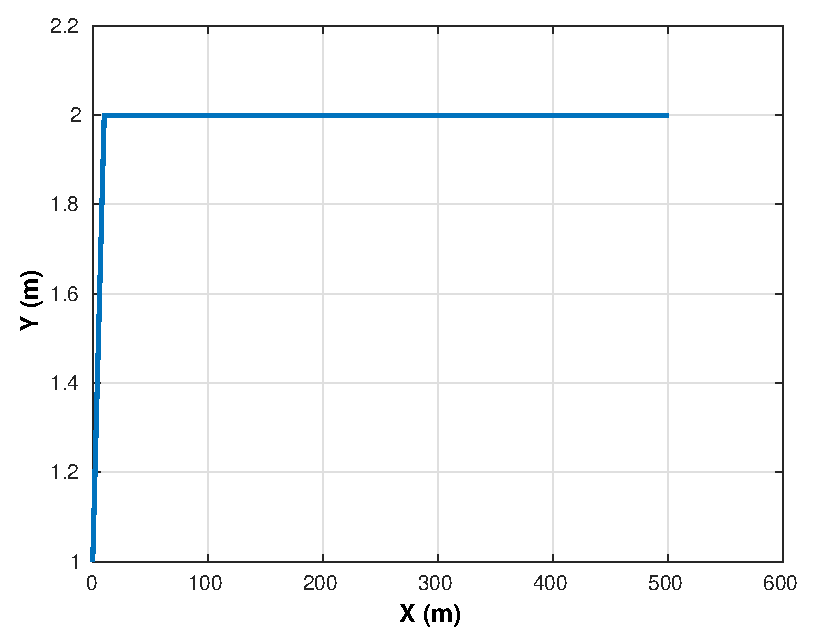
\includegraphics [width=4in]{vehicle_steering_04.eps}



\end{document}
    
